\section{ChimeraX Operate protocol}
\label{app:chimeraOperate}%a020

Protocol designed to perform operations with atomic structures in \scipion by using \chimera. A volume or set of volumes can also be included. Structures or maps generated by using this protocol can be saved in \scipion after executing specific \chimera commands. \chimera \ttt{rigid fit} protocol constitutes a particular case of this protocol to perform rigid fitting in \scipion by using \chimera (Appendix \ref{app:chimeraRigidFit}).

 \begin{itemize}
  \item Requirements to run this protocol and visualize results:
                \begin{itemize}
                    \item \scipion plugin: \ttt{scipion-em}
                    \item \scipion plugin: \ttt{scipion-em-chimera}
                \end{itemize}
  \item \scipion menu:\\
                \ttt{Model building -> Tools-Calculators} (\ffigure{fig:app_protocol_chimera_2} (A))
  
  \item Protocol form parameters (\ffigure{fig:app_protocol_chimera_2} (B)):
  
                \begin{figure}[H]
                \centering 
                \captionsetup{width=.7\linewidth} 
                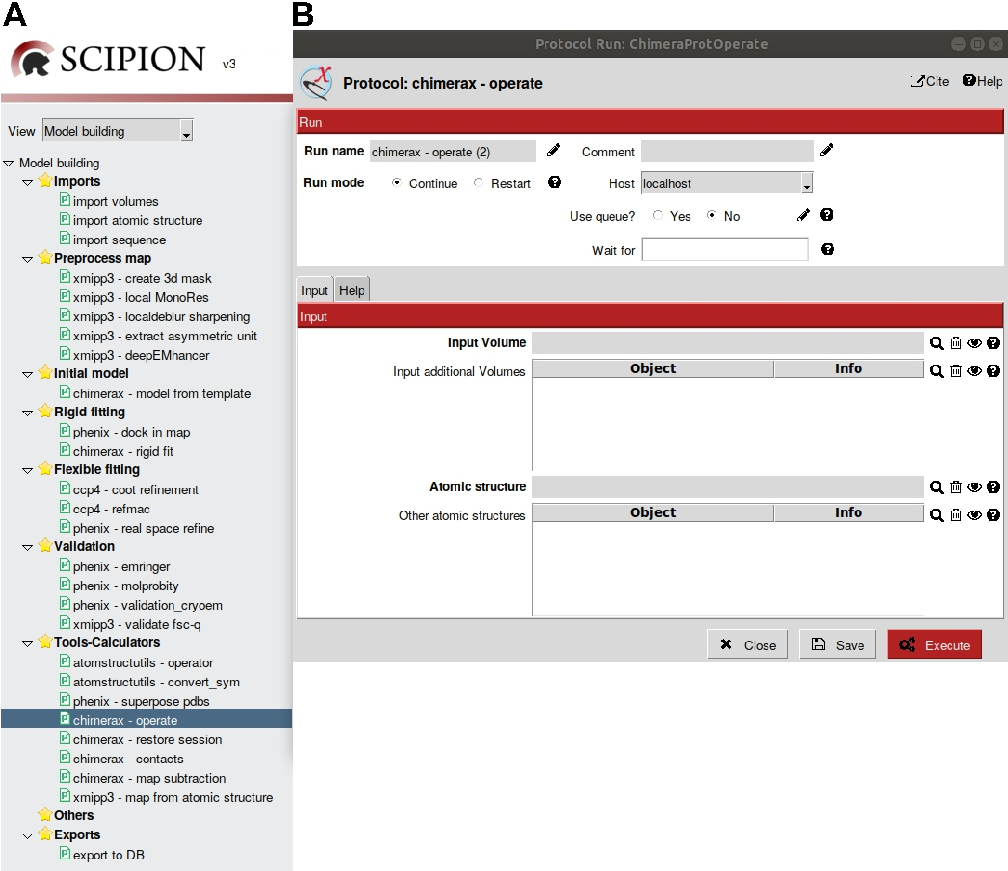
\includegraphics[width=0.90\textwidth]{Images_appendix/Fig117.pdf}
                \caption{Protocol \scommand{chimerax - operate}. A: Protocol location in \scipion menu. B: Protocol form.}
                \label{fig:app_protocol_chimera_2}
                \end{figure}
    
                \begin{itemize}
                \item \ttt{Input} section

                                \begin{itemize}
                                \item \ttt{Input Volume}: Optional parameter to be completed with the electron density map previously downloaded or generated in \scipion.
                                \item \ttt{Input additional Volumes}: Optional parameter to include other electron density maps previously downloaded or generated in \scipion.
                                \item \ttt{Atomic structure}: Atomic structure previously downloaded or generated in \scipion.
                                \item \ttt{Other atomic structures}: Additional atomic structures.
                                \end{itemize}
                \item \ttt{Help} section
                    
                                This section contains \chimera commands required to save $models$ according to their reference volumes, which can also be saved if required. Remark that using \ttt{scipionwrite} command, \chimera session will be saved by default, without prejudice that it may be saved with \ttt{scipionss} command. \ttt{scipioncombine} command allows to merge in only one atomic structure two or more. \chimera sessions can be restored by using \scommand{chimerax - restore session} protocol.
                    
                \end{itemize}

  \item Protocol execution:\\
  
                Adding specific protocol label is recommended in \ttt{Run name} section, at the form top. To add the label, open the protocol form, press the pencil symbol at the right side of \ttt{Run name} box, complete the label in the new opened window, press OK and, finally, close the protocol. This label will be shown in the output summary content (see below). If you want to run again this protocol, do not forget to set to \ttt{Restart} the \ttt{Run mode}.\\
                Press the \ttt{Execute} red button at the form bottom.\\
                
                \chimera graphics window will be opened after executing the protocol. Electron density map(s), if loaded, and the atomic structure(s) are shown. Steps to follow depend on the specific operation to carry out. Usually, new volumes or structures are generated, sometimes by combination of others, each one with a specific $model$ number displayed in the \ttt{Models} panel, and they have to be saved in \scipion.
                            \begin{itemize}
                            
                            \item To combine two or more atomic structures:\\
                            Write in \chimera command line:\\
                            \ttt{scipioncombine \#n1,n2}\\
                            \\
                            \ttt{\#n1} and \ttt{\#n2} are the respective $model$ numbers of two different atomic structures. Optionally you can set the $model$ number of the output combined structure \ttt{\#n3}:\\
                            \ttt{scipioncombine \#n1,n2 modelid n3}\\
                            \item To save a map or an atomic structure generated with this \chimera protocol with $model$ number \ttt{\#n}:\\
                            Write in \chimera command line:\\
                            \ttt{scipionwrite \#n}\\
                            \\
                            Optionally you can write a prefix to easily recognize that map or structure. Then, the prefix depends on the user. Example:\\
                            \ttt{scipionwrite \#n prefix my\_favorite\_model\_}\\
                            
                            \item Close \chimera graphics window.

                            \end{itemize}
  \item Visualization of protocol results:
  
                After executing the protocol, press \ttt{Analyze Results} and \chimera graphics window will be opened by default. Atomic structures and volumes are referred to the origin of coordinates in \chimera. To show the relative position of atomic structures and electron density volumes, the three coordinate axes are represented; X axis (red), Y axis (yellow), and Z axis (blue) (\ffigure{fig:app_protocol_volume_3}). Coordinate axes, volume, and atomic structure are model numbers \ttt{\#1}, \ttt{\#2}, and \ttt{\#3}, respectively, in \chimera \ttt{Models} panel. If no volumes have been included, coordinate axes and each atomic structure are model numbers \ttt{\#1} and \ttt{\#2}, respectively.
                
                \begin{figure}[H]
                \centering 
                \captionsetup{width=.9\linewidth} 
                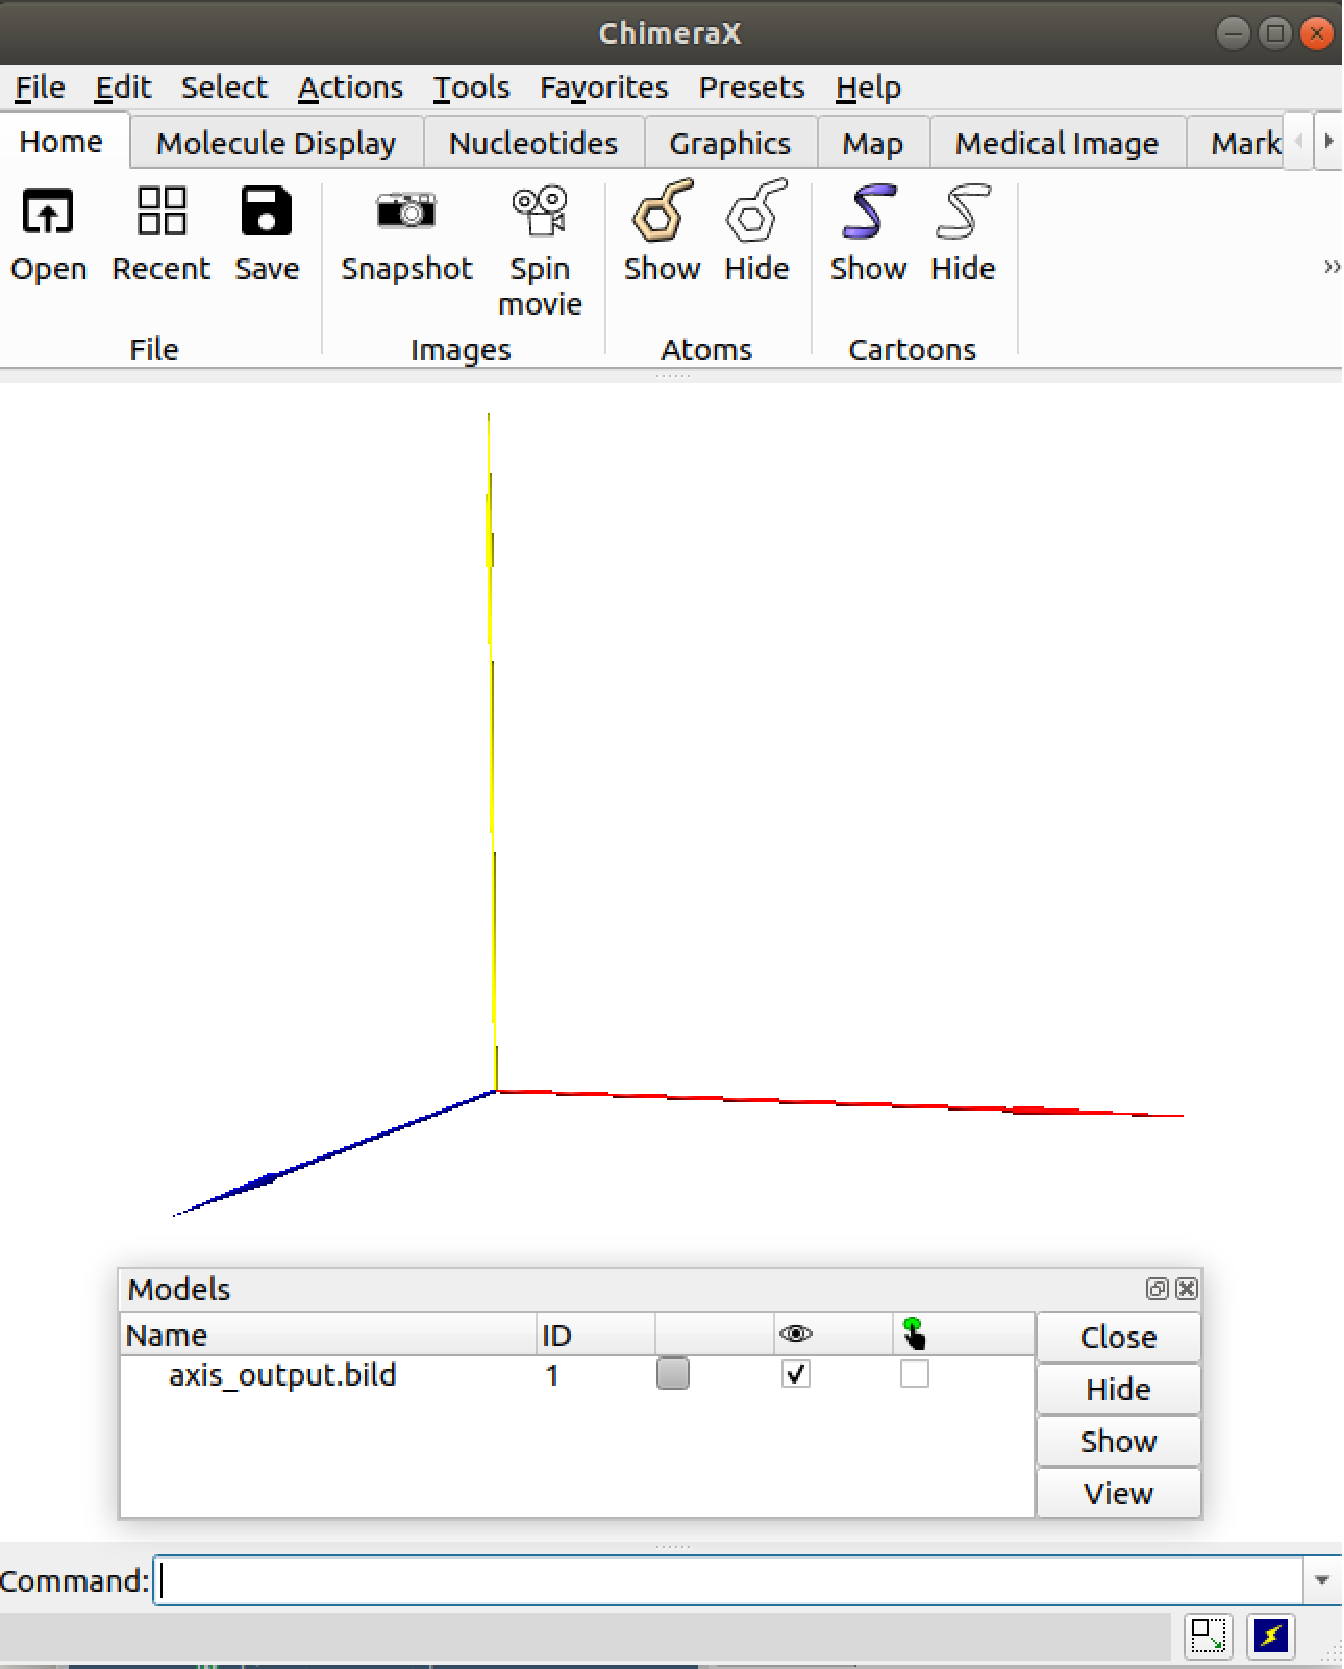
\includegraphics[width=0.5\textwidth]{Images_appendix/Fig102.pdf}
                \caption{Default $ChimeraX$ graphics window with coordinate axes.}
                \label{fig:app_protocol_volume_3}
                \end{figure}
   
  \item Summary content:\\
  
                \begin{itemize}
                    \item If an atomic structure is generated:

                                \begin{itemize}
                                \item Protocol output (below \scipion framework):\\
                                        \ttt{chimerax - operate -> output atomic structure name, starting with the prefix};\\ \ttt{AtomStruct (pseudoatoms=True/ False, volume=True/ False)}.\\Pseudoatoms is set to \ttt{True} when the structure is made of pseudoatoms instead of atoms. Volume is set to \ttt{True} when an electron density map is associated to the atomic structure.
                                \item \ttt{SUMMARY} box:\\Produced files:\\output atomic structure name, starting with the prefix (.cif file)\\we have some result
                                \end{itemize}
                    \item If a volume is generated:
                    
                                \begin{itemize}
                                \item Protocol output (below \scipion framework):\\
                                        \ttt{chimerax - operate -> output 3D map name}; \ttt{Volume (x, y, and z dimensions, sampling rate)}.\\
                                \item \ttt{SUMMARY} box:\\Produced files:\\output 3D map name, starting with the prefix (.mrc file)\\we have some result
                                \end{itemize}
                    
                \end{itemize}
  
 \end{itemize}

